%% LyX 2.2.2 created this file.  For more info, see http://www.lyx.org/.
%% Do not edit unless you really know what you are doing.
\documentclass[ruled]{article}
\usepackage{courier}
\usepackage[T1]{fontenc}
\usepackage[latin9]{inputenc}
\usepackage[letterpaper]{geometry}
\geometry{verbose}
\usepackage{color}
\usepackage{algorithm2e}
\usepackage{amsmath}
\usepackage{amssymb}
\usepackage{graphicx}
\usepackage[unicode=true,
 bookmarks=false,
 breaklinks=false,pdfborder={0 0 1},backref=section,colorlinks=true]
 {hyperref}
\usepackage{minted}
\makeatletter

%%%%%%%%%%%%%%%%%%%%%%%%%%%%%% LyX specific LaTeX commands.
\providecommand{\LyX}{\texorpdfstring%
  {L\kern-.1667em\lower.25em\hbox{Y}\kern-.125emX\@}
  {LyX}}
%% Because html converters don't know tabularnewline
\providecommand{\tabularnewline}{\\}

\@ifundefined{date}{}{\date{}}
%%%%%%%%%%%%%%%%%%%%%%%%%%%%%% User specified LaTeX commands.
\definecolor{mygreen}{rgb}{0,0.6,0}
\definecolor{mygray}{rgb}{0.5,0.5,0.5}
\definecolor{mymauve}{rgb}{0.58,0,0.82}

\makeatother

\usepackage{listings}
\lstset{backgroundcolor={\color{white}},
basicstyle={\footnotesize\ttfamily},
breakatwhitespace=false,
breaklines=true,
captionpos=b,
commentstyle={\color{mygreen}},
deletekeywords={...},
escapeinside={\%*}{*)},
extendedchars=true,
frame=shadowbox,
keepspaces=true,
keywordstyle={\color{blue}},
language=Python,
morekeywords={*,...},
numbers=none,
numbersep=5pt,
numberstyle={\tiny\color{mygray}},
rulecolor={\color{black}},
showspaces=false,
showstringspaces=false,
showtabs=false,
stepnumber=1,
stringstyle={\color{mymauve}},
tabsize=2}
\begin{document}
\global\long\def\reals{\mathbf{R}}
 \global\long\def\integers{\mathbf{Z}}
\global\long\def\naturals{\mathbf{N}}
 \global\long\def\rationals{\mathbf{Q}}
\global\long\def\ca{\mathcal{A}}
\global\long\def\cb{\mathcal{B}}
 \global\long\def\cc{\mathcal{C}}
 \global\long\def\cd{\mathcal{D}}
\global\long\def\ce{\mathcal{E}}
\global\long\def\cf{\mathcal{F}}
\global\long\def\cg{\mathcal{G}}
\global\long\def\ch{\mathcal{H}}
\global\long\def\ci{\mathcal{I}}
\global\long\def\cj{\mathcal{J}}
\global\long\def\ck{\mathcal{K}}
\global\long\def\cl{\mathcal{L}}
\global\long\def\cm{\mathcal{M}}
\global\long\def\cn{\mathcal{N}}
\global\long\def\co{\mathcal{O}}
\global\long\def\cp{\mathcal{P}}
\global\long\def\cq{\mathcal{Q}}
\global\long\def\calr{\mathcal{R}}
\global\long\def\cs{\mathcal{S}}
\global\long\def\ct{\mathcal{T}}
\global\long\def\cu{\mathcal{U}}
\global\long\def\cv{\mathcal{V}}
\global\long\def\cw{\mathcal{W}}
\global\long\def\cx{\mathcal{X}}
\global\long\def\cy{\mathcal{Y}}
\global\long\def\cz{\mathcal{Z}}
\global\long\def\ind#1{1(#1)}
\global\long\def\pr{\mathbb{P}}

\global\long\def\ex{\mathbb{E}}
\global\long\def\var{\textrm{Var}}
\global\long\def\cov{\textrm{Cov}}
\global\long\def\sgn{\textrm{sgn}}
\global\long\def\sign{\textrm{sign}}
\global\long\def\kl{\textrm{KL}}
\global\long\def\law{\mathcal{L}}
\global\long\def\eps{\varepsilon}
\global\long\def\convd{\stackrel{d}{\to}}
\global\long\def\eqd{\stackrel{d}{=}}
\global\long\def\del{\nabla}
\global\long\def\loss{\ell}
\global\long\def\tr{\operatorname{tr}}
\global\long\def\trace{\operatorname{trace}}
\global\long\def\diag{\text{diag}}
\global\long\def\rank{\text{rank}}
\global\long\def\linspan{\text{span}}
\global\long\def\proj{\text{Proj}}
\global\long\def\argmax{\operatornamewithlimits{arg\, max}}
\global\long\def\argmin{\operatornamewithlimits{arg\, min}}
\global\long\def\bfx{\mathbf{x}}
\global\long\def\bfy{\mathbf{y}}
\global\long\def\bfl{\mathbf{\lambda}}
\global\long\def\bfm{\mathbf{\mu}}
\global\long\def\calL{\mathcal{L}}
\global\long\def\vw{\boldsymbol{w}}
\global\long\def\vx{\boldsymbol{x}}
\global\long\def\vxi{\boldsymbol{\xi}}
\global\long\def\valpha{\boldsymbol{\alpha}}
\global\long\def\vbeta{\boldsymbol{\beta}}
\global\long\def\vsigma{\boldsymbol{\sigma}}
\global\long\def\vmu{\boldsymbol{\mu}}
\global\long\def\vtheta{\boldsymbol{\theta}}
\global\long\def\vd{\boldsymbol{d}}
\global\long\def\vs{\boldsymbol{s}}
\global\long\def\vt{\boldsymbol{t}}
\global\long\def\vh{\boldsymbol{h}}
\global\long\def\ve{\boldsymbol{e}}
\global\long\def\vf{\boldsymbol{f}}
\global\long\def\vg{\boldsymbol{g}}
\global\long\def\vz{\boldsymbol{z}}
\global\long\def\vk{\boldsymbol{k}}
\global\long\def\va{\boldsymbol{a}}
\global\long\def\vb{\boldsymbol{b}}
\global\long\def\vv{\boldsymbol{v}}
\global\long\def\vy{\boldsymbol{y}}


\title{Machine Learning and Computational Statistics\\
Homework 7: Bayesian Statistics}

\maketitle
\textbf{Due: Monday, May 15, 2017, at 10pm (Submit via Gradescope)}

\textbf{Instructions}: Your answers to the questions below, including
plots and mathematical work, should be submitted as a single PDF file.
It's preferred that you write your answers using software that typesets
mathematics (e.g. \LaTeX{}, \LyX{}, or MathJax via iPython), though
if you need to you may scan handwritten work. You may find the \href{https://github.com/gpoore/minted}{minted}
package convenient for including source code in your \LaTeX{} document.
If you are using \LyX{}, then the \href{https://en.wikibooks.org/wiki/LaTeX/Source_Code_Listings}{listings}
package tends to work better.

\section{Introduction }

In this homework we work through several basic concepts in Bayesian
statistics via one of the simplest problems there is: estimating the
probability of heads in a coin flip. Later we'll extend this to the
probability of estimating click-through rates in mobile advertising.

\section{Coin Flipping: Maximum Likelihood}
\begin{enumerate}
\item Suppose we flip a coin and get the following sequence of heads and
tails:
\[
\cd=(H,H,T)
\]
Give an expression for the probability of observing $\cd$ given that
the probability of heads is $\theta$. That is, give an expression
for $p\left(\cd\mid\theta\right)$. This is called the \textbf{likelihood
of $\theta$ for the data $\cd$}.\\
\noindent\rule{14.3cm}{2pt}\\
\textbf{Answer:}\\
\[
p(\cd \mid \theta)=\theta^2(1-\theta)
\]
\pagebreak
\item How many different sequences of 3 coin tosses have $2$ heads and
1 tail? If we coss the coin $3$ times, what is the probability of
2 heads and $1$ tail? (Answer should be in terms of $\theta$.)\\
\noindent\rule{14.3cm}{2pt}\\
\textbf{Answer:}\\
There exists 3 different sequences that contain 2 heads and 1 tail. $(H,H,T)$,$ (H,T,H)$ and $(T,H,T)$.
The probability of observing 2 heads and 1 tail is: $3\theta^2(1-\theta)$

\pagebreak
\item More generally, give an expression for the likelihood $p(\cd\mid\theta)$
for a particular sequence of flips $\cd$ that has $n_{h}$ heads
and $n_{t}$ tails. Make sure you have expressions that make sense
even for $\theta=0$ and $n_{h}=0$, and other boundary cases. You
may use the convention that $0^{0}=1$, or you can break your expression
into cases if needed.\\
\noindent\rule{14.3cm}{2pt}\\
\textbf{Answer:}\\
We take the order of a sequence into account, therefore:
\[
p(\cd \mid \theta) =  \theta^{n_h}(1-\theta)^{n_t}
\]

\pagebreak
\item Prove that the maximum likelihood estimate of $\theta$ given we observed
a sequence with $n_{h}$ heads and $n_{t}$ tails is
\[
\hat{\theta}_{\text{MLE}}=\frac{n_{h}}{n_{h}+n_{t}}.
\]
You may assume that $n_{h}+n_{t}\ge1$. (Hint: Maximizing the log-likelihood
is equivalent and is often easier. )\\
\noindent\rule{14.3cm}{2pt}\\
\textbf{Answer:}\\
From part 3, we have $p(\cd \mid \theta) = \binom{n_h+n_t}{n_h} \theta^{n_h}(1-\theta)^{n_t}$. Take the derivative of $\log p(\cd \mid \theta)$ yields:
\begin{align}
\frac{\partial \log p(\cd \mid \hat{\theta}_{\text{MLE}})}{\partial \theta} =0 \implies \frac{n_h}{\hat{\theta}_{\text{MLE}}}-\frac{n_t}{(1-\hat{\theta}_{\text{MLE}})}&=0\\
\hat{\theta}_{\text{MLE}}&=\frac{n_h}{n_h+n_t}
\end{align}
\pagebreak

\end{enumerate}

\section{Coin Flipping: Bayesian Approach with Beta Prior}

We'll now take a Bayesian approach to the coin flipping problem, in
which we treat $\theta$ as a random variable sampled from some prior
distribution $p(\theta)$. We'll represent the $i$th coin flip by
a random variable $X_{i}\in\left\{ 0,1\right\} $, where $X_{i}=1$
if the $i$th flip is heads. We assume that the $X_{i}$'s are conditionally
indendent given $\theta$. This means that the joint distribution
of the coin flips and $\theta$ factorizes as follows:
\begin{eqnarray*}
p(x_{1},\ldots,x_{n},\theta) & = & p(\theta)p(x_{1},\ldots,x_{n}\mid\theta)\mbox{ (always true)}\\
 & = & p(\theta)\prod_{i=1}^{n}p(x_{i}\mid\theta)\text{ (by conditional independence).}
\end{eqnarray*}

\begin{enumerate}
\item Suppose that our prior distribution on $\theta$ is $\mbox{Beta}(h,t)$,
for some $h,t>0$. That is, $p(\theta)\propto\theta^{h-1}\left(1-\theta\right)^{t-1}$.
Suppose that our sequence of flips $\cd$ has $n_{h}$ heads and $n_{t}$
tails. Show that the posterior distribution for $\theta$ is $\mbox{Beta}(h+n_{h},t+n_{t})$.
That is, show that
\[
p(\theta\mid\cd)\propto\theta^{h-1+n_{h}}\left(1-\theta\right)^{t-1+n_{t}}.
\]
 We say that the Beta distribution is \textbf{conjugate} to the Bernoulli
distribution since the prior and the posterior are both in the same
family of distributions (i.e. both Beta distributions).\\
\noindent\rule{14.3cm}{2pt}\\
\textbf{Answer:}\\
\begin{align*}
p(\theta \mid \cd) \propto p(\theta)p(\cd \mid \theta) &= \theta^{h-1}\left(1-\theta\right)^{t-1} \theta^{n_h}(1-\theta)^{n_t}\\
&=\theta^{h-1+n_{h}}\left(1-\theta\right)^{t-1+n_{t}}
\end{align*}

\pagebreak
\item Give expressions for the MLE, the MAP, and the posterior mean estimates
of $\theta$. {[}Hint: You may use the fact that a $\mbox{Beta}(h,t)$
distribution has mean $h/(h+t)$ and has mode $\left(h-1\right)/\left(h+t-2\right)$
for $h,t>1$. For the Bayesian solutions, you should note that as
$h+t$ gets very large, and assuming we keep the ratio $h/(h+t)$
fixed, the posterior mean and MAP approach the prior mean $h/\left(h+t\right)$,
while for fixed $h$ and $t$, the posterior mean approaches the MLE
as the sample size $n=n_{h}+n_{t}\to\infty$.\\
\noindent\rule{14.3cm}{2pt}\\
\textbf{Answer:}\\
The maximum likelihood estimation $\theta_{\text{MLE }}$ should be the mode of likelihood function: $p(\cd \mid \theta) =\binom{n_h+n_t}{n_h} \theta^{n_h}(1-\theta)^{n_t}$, and should have zero derivative at $\theta_{\text{MLE}}$:
\[
\frac{\partial p(\cd \mid \theta)}{\theta} = 0 \implies \theta_{\text{MLE}}=\frac{n_h}{n_h+n_t}
\]
\\
From part 1, we have $p(\theta \mid \cd) \propto \theta^{h-1+n_{h}}\left(1-\theta\right)^{t-1+n_{t}}=Beta(n_h+h,n_t+t)$. The MAP estimation$\theta_{\text{MAP}}$ should be the mode of posterior distribution:
\[
\hat{\theta}_{\text{MAP}} = \frac{n_h+h-1}{n_h+h+n_t+t-2}
\]
The posterior mean of $\theta$ is:
\[
\hat{\theta}_{\text{POSTERIOR MEAN}}=\frac{n_h+h}{n_h+h+n_t+t}
\]

\pagebreak
\item What happens to $\hat{\theta}_{\text{MLE }}$, $\hat{\theta}_{\text{MAP}}$,
and $\hat{\theta}_{\text{POSTERIOR MEAN}}$ as the number of coin
flips $n=n_{h}+n_{t}$ approaches infinity? \\
\noindent\rule{14.3cm}{2pt}\\
\textbf{Answer:}\\
When $n$ approaches infinity, the effect of prior on posterior is negligible. Therefore we expect $\hat{\theta}_{\text{MAP}}$,
and $\hat{\theta}_{\text{POSTERIOR MEAN}}$ to converges to $\theta$. By the definition of $\hat{\theta}_{\text{MLE }}$, the variance of $\hat{\theta}_{\text{MLE }}$ would be decrease with the increase of $n$ and finally converges to $\theta$.

\pagebreak
\item The MAP and posterior mean estimators of $\theta$ were derived from
a Bayesian perspective. Let's now evaluate them from a frequentist
perspective. Suppose $\theta$ is fixed and unknown. Which of the
MLE, MAP, and posterior mean estimators give \textbf{unbiased} estimates
of $\theta$, if any? {[}Hint: The answer may depend on the parameters
$h$ and $t$ of the prior. Also, let's consider the total number
of flips $n=n_{h}+n_{t}$ to be given (not random), while $n_{h}$
and $n_{t}$ are random, with $n_{h}=n-n_{t}$.{]}\\
\noindent\rule{14.3cm}{2pt}\\
\textbf{Answer:}\\
$\hat{\theta}_{\text{MLE}}$ is unbiased because:
\[
\mathbb{E}[\hat{\theta}_{\text{MLE}}]=\mathbb{E}[\frac{n_h}{n}] = \frac{1}{n}\mathbb{E}[n_h] = \frac{n\theta}{n} = \theta
\]
 $\hat{\theta}_{\text{MAP}}$ could be biased, since:
 \[
 \mathbb{E}[ \hat{\theta}_{\text{MAP}}] = \mathbb{E}[\frac{n_h+h-1}{n+h+t-2}]=\frac{n\theta+h-1}{n+h+t-2}]
 \]
 $\hat{\theta}_{\text{MAP}}$ is unbiased only when h=t=1.\\
$\hat{\theta}_{\text{POSTERIOR MEAN}}$ is biased since:
\[
\mathbb{E}[\hat{\theta}_{\text{POSTERIOR MEAN}}]=\mathbb{E}[\frac{n_h+h}{n+h+t}]=\mathbb{E}[\frac{n\theta+h}{n+h+t}]
\]
$\hat{\theta}_{\text{POSTERIOR MEAN}}$ is unbiased only when h=t=0. But h and t cannot be zero. 
\pagebreak
\item Suppose somebody gives you a coin and asks you to give an estimate
of the probability of heads, but you can only toss the coin $3$ times.
You have no particular reason to believe this is an unfair coin. Would
you prefer the MLE or the posterior mean as a point estimate of $\theta$?
If the posterior mean, what would you use for your prior?\\
\noindent\rule{14.3cm}{2pt}\\
\textbf{Answer:}\\
I would prefer posterior mean. Because for 3 coins tosses, $\hat{\theta}_{\text{MLE}}$ is very instable. For example if you get three heads, $\hat{\theta}_{\text{MLE}}=1$. But the results of three heads is totally observable even with a fair coin. \\
If I chose posterior mean, I would choose prior that have mode in $\theta=\frac{1}{2}$ since I don't have a particular reason to believe this is an unfair coin. But I am not that sure it is a fair coin either. Therefore I choose Beta(2,2) as my prior. 
\end{enumerate}

\pagebreak
\section{Hierarchical Bayes for Click-Through Rate Estimation}

In mobile advertising, ads are often displayed inside apps on a phone
or tablet device. When an ad is displayed, this is called an ``impression.''
If the user clicks on the ad, that is called a ``click.'' The probability
that an impression leads to a click is called the ``click-through
rate'' (CTR). 

Suppose we have $d=1000$ apps. For various reasons\footnote{The primary reason is that different apps place the ads differently,
making it more or less difficult to avoid clicking the ad.}, each app tends to have a different overall CTR. For the purposes
of designing an ad campaign, we want estimates of all the app-level
CTRs, which we'll denote by $\theta_{1},\ldots,\theta_{1000}$. Of
course, the particular user seeing the impression and the particular
ad that is shown have an effect on the CTR, but we'll ignore these
issues for now. {[}Because so many clicks on mobile ads are accidental,
it turns out that the overall app-level CTR often dominates the effect
of the particular user and the specific ad.{]} 

If we have enough impressions for a particular app, then the empirical
fraction of clicks will give a good estimate for the actual CTR. However,
if we have relatively few impressions, we'll have some problems using
the empirical fraction. Typical CTRs are less than 1\%, so it takes
a fairly large number of observations to get a good estimate of CTR.
For example, even with $100$ impressions, the only possible CTR estimates
given by the MLE would be $0\%,1\%,2\%,\ldots,100\%$. The $0\%$
estimate is almost certainly much too low, and anything $2\%$ or
higher is almost certainly much too high. Our goal is to come up with
reasonable point estimates for $\theta_{1},\ldots,\theta_{1000}$,
even when we have very few observations for some apps. 

If we wanted to apply the Bayesian approach worked out in the previous
problem, we could come up with a prior that seemed reasonable. For
example, we could use the following $\mbox{Beta}(3,400)$ as a prior
distribution on each $\theta_{i}$:
\begin{center}
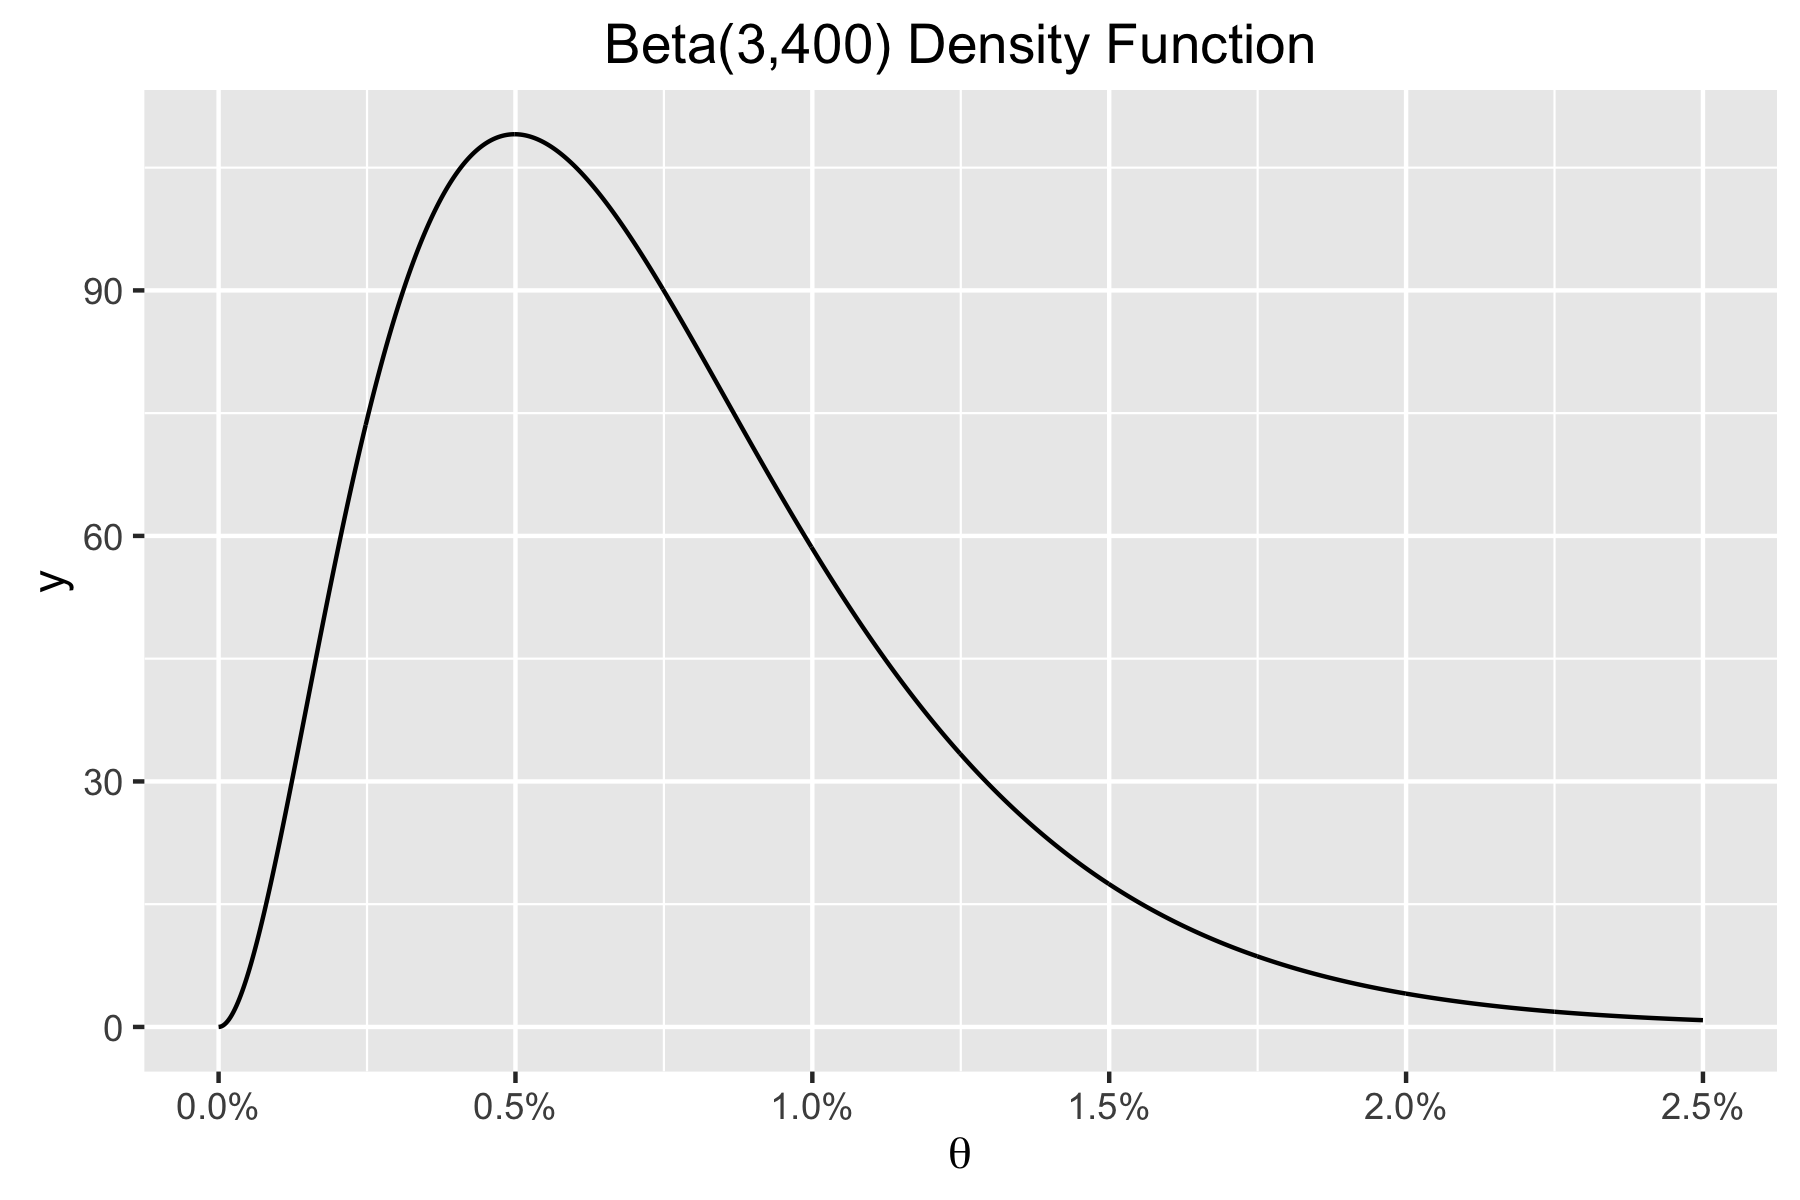
\includegraphics[height=2in]{figures/beta3-400}
\par\end{center}

In this basic Bayesian approach, the parameters $3$ and $400$ would
be chosen by the data scientist based on prior experience, or ``best
guess'', but without looking at the new data. Another approach would
be to use the data to help you choose the parameters $a$ and $b$
in $\mbox{Beta}(a,b)$. This would \textbf{not} be a Bayesian approach,
though it is frequently used in practice. One method in this direction
is called \textbf{empirical Bayes}. Empirical Bayes can be considered
a frequentist approach, in which we estimate $a$ and $b$ from the
data $\cd$ using some estimation technique, such as maximum likelihood.
The proper Bayesian approach to this type of thing is called \textbf{hierarchical
Bayes}, in which we put another prior distribution on $a$ and $b$.
We'll investigate each of these approaches below. 

\subsubsection*{Mathematical Description}

We'll now give a mathematical description of our model, assuming the
prior parameters $a$ and $b$ are directly chosen by the data scientist.
Let $n_{1},\ldots,n_{d}$ be the number of impressions we observe
for each of the $d$ apps. In this problem, we will not consider these
to be random numbers. For the $i$th app, let $c_{i}^{1},\ldots,c_{i}^{n_{i}}\in\left\{ 0,1\right\} $
be indicator variables determining whether or not each impression
was clicked. That is, $c_{i}^{j}=\ind{j\mbox{th impression on }i\mbox{th app was clicked}}$.
We can summarize the data on the $i$th app by $\cd_{i}=\left(x_{i},n_{i}\right)$,
where $x_{i}=\sum_{j=1}^{n_{i}}c_{i}^{j}$ is the total number of
impressions that were clicked for app $i$. Let $\theta=(\theta_{1},\ldots,\theta_{d})$,
where $\theta_{i}$ is the CTR for app $i$. 

In our Bayesian approach, we act as though the data were generated
as follows:
\begin{enumerate}
\item Sample $\theta_{1},\ldots,\theta_{d}$ i.i.d. from Beta$(a,b)$. 
\item For each app $i$, sample $c_{i}^{1},\ldots,c_{i}^{n_{i}}$ i.i.d.
from Bernoulli$(\theta_{i})$. 
\end{enumerate}

\subsection{\label{subsec:Empirical-Bayes-single-app}Empirical Bayes for a single
app}

We start by working out some details for Bayesian inference for a
single app. That is, suppose we only have the data $\cd_{i}$ from
app $i$, and nothing else. Mathematically, this is exactly the same
setting as the coin tossing setting above, but here we push it further.
\begin{enumerate}
\item Give an expression for $p(\cd_{i}\mid\theta_{i})$, the likelihood
of $\cd_{i}$ given the probability of click $\theta_{i}$, in terms
of $\theta_{i}$, $x_{i}$ and $n_{i}$.\\
\noindent\rule{14.3cm}{2pt}
\\
\textbf{Answer:}
\[
p(\cd_i \mid \theta_i) =  \theta^{x_i}(1-\theta)^{n_i-x_i}
\]

\pagebreak
\item We will take our prior distribution on $\theta_{i}$ to be $\mbox{Beta}(a,b)$.
The correpoding probability density function is given by
\[
p(\theta_{i})=\mbox{Beta}(\theta_{i};a,b)=\frac{1}{B(a,b)}\theta_{i}^{a-1}\left(1-\theta_{i}\right)^{b-1},
\]
where $B(a,b)$ is called the Beta function. Explain (without calculation)
why we must have
\[
\int\theta_{i}^{a-1}\left(1-\theta_{i}\right)^{b-1}\,d\theta_{i}=B(a,b).
\]
\\
\noindent\rule{14.3cm}{2pt}
\\
\textbf{Answer:}\\
Because $p(\theta_{i})$ is defined to be a probability density function and therefore we should have $\int p(\theta_i) d\theta_i=1$
\pagebreak
\item Give an expression for the posterior distribution $p(\theta_{i}\mid\cd_{i})$.
In this case, include the constant of proportionality. In other words,
do not use the ``is proportional to'' sign $\propto$ in your final
expression. You \textbf{may }reference the Beta function defined above.
{[}Hint: This problem is essentially a repetition of an earlier problem.{]} 
\\
\noindent\rule{14.3cm}{2pt}
\\
\textbf{Answer:}\\
\begin{align}
p(\theta_i \mid \cd_{i})&\propto p(\cd \mid \theta_i)p(\theta_i)\\
&=\frac{\theta_i^{x_i+a-1}(1-\theta_i)^{n-x_i+b-1}}{B(a,b)}\\
&\propto \theta_i^{x_i+a-1}(1-\theta_i)^{n-x_i+b-1}\\
\end{align}
We know that $p(\theta_i \mid \cd)$is a probability density function, therefore we must have $\int p(\theta_i \mid \cd_i)=1$. Combined with conclusion of part 2, we have:

\begin{equation}
p(\theta_i \mid \cd_i) = \frac{\theta_i^{x_i+a-1}(1-\theta_i)^{n-x_i+b-1}}{B(x_i+a,n-xi+b)}
\end{equation}
\pagebreak
\item Give a closed form expression for $p(\cd_{i})$, the marginal likelihood
of $\cd_{i}$, in terms of the $a,b,x_{i},$ and $n_{i}$. You may
use the normalization function $B(\cdot,\cdot)$ for convenience,
but you should not have any integrals in your solution. (Hint: $p(\cd_{i})=\int p\left(\cd_{i}\mid\theta_{i}\right)p(\theta_{i})\,d\theta_{i}$,
and the answer will be a ratio of two beta function evaluations.)
\\
\noindent\rule{14.3cm}{2pt}
\\
\textbf{Answer:}\\
\begin{align}
p(\cd_i)&=\int_0^1 p(\cd_{i} \mid \theta_{i})p(\theta_i)d\theta_i\\
&=\frac{1}{B(a,b)}\int_0^1 \theta^{x_i+a-1}(1-\theta)^{n_i-x_i+b-1}\\
&=\frac{B(x_i+a,n_i-x_i+b)}{B(a,b)}
\end{align}
\pagebreak
\item The maximum likelihood estimate for $\theta_{i}$ is $x_{i}/n_{i}$.
Let $p_{\text{MLE}}(\cd_{i})$ be the marginal likelihood of $\cd_{i}$
when we use a prior on $\theta_{i}$ that puts all of its probability
mass at $x_{i}/n_{i}$. Note that 
\begin{eqnarray*}
p_{\text{MLE}}(\cd_{i}) & = & p\left(\cd_{i}\mid\theta_{i}=\frac{x_{i}}{n_{i}}\right)p\left(\theta_{i}=\frac{x_{i}}{n_{i}}\right)\\
 & = & p\left(\cd_{i}\mid\theta_{i}=\frac{x_{i}}{n_{i}}\right).
\end{eqnarray*}
Explain why, or prove, that $p_{\text{MLE}}(\cd_{i})$ is larger than
$p(\cd_{i})$ for any other prior we might put on $\theta_{i}$. If
it's too hard to reason about all possible priors, it's fine to just
consider all Beta priors. {[}Hint: This does not require much or any
calculation. It may help to think about the integral $p(\cd_{i})=\int p\left(\cd_{i}\mid\theta_{i}\right)p(\theta_{i})\,d\theta_{i}$
as a weighted average of $p(\cd_{i}\mid\theta_{i})$ for different
values of $\theta_{i}$, where the weights are $p(\theta_{i})$.{]}
\\
\noindent\rule{14.3cm}{2pt}
\\
\textbf{Answer:}\\
By the definition of MLE, we must have $p(\cd_i \mid \theta)\leq p(\cd_i \mid \theta_{\text{MLE}})$. Therefore:

\begin{align}
p(\cd_i) &= \int p(\cd_i \mid \theta_i)p(\theta_i) d\theta\\
&\leq \int p(\cd_i \mid \theta_{\text{MLE}}) p(\theta_i) d\theta\\
&=p(\cd_i \mid \theta_{\text{MLE}})  \int p(\theta_i)d\theta\\
&=p(\cd_i \mid \theta_{\text{MLE}}) 
\end{align}
Since $p(\theta)$ is a probability density distribution.
\pagebreak
\item One approach to getting an \textbf{empirical Bayes} estimate of the
parameters $a$ and $b$ is to use maximum likelihood. Such an empirical
Bayes estimate is often called an \textbf{ML-2} estimate, since it's
maximum likelihood, but at a higher level in the Bayesian hierarchy.
To emphasize the dependence of the likelihood of $\cd_{i}$ on the
parameters $a$ and $b$, we'll now write it as $p(\cd_{i}\mid a,b)$\footnote{Note that this is a slight (though common) abuse of notation, because
$a$ and $b$ are not random variables in this setting. It might be
more appropriate to write this as $p(\cd_{i};a,b)$ or $p_{a,b}(\cd_{i})$.
But this isn't very common.}. The empirical Bayes estimates for $a$ and $b$ are given by
\[
(\hat{a},\hat{b})=\argmax_{\left(a,b\right)\in\reals^{>0}\times\reals^{>0}}p(\cd_{i}\mid a,b).
\]
To make things concrete, suppose we observed $x_{i}=3$ clicks out
of $n_{i}=500$ impressions. A plot of $p(\cd_{i}\mid a,b)$ as a
function of $a$ and $b$ is given in Figure \ref{fig:single-app-contour-plot}.
\begin{figure}
\centering{}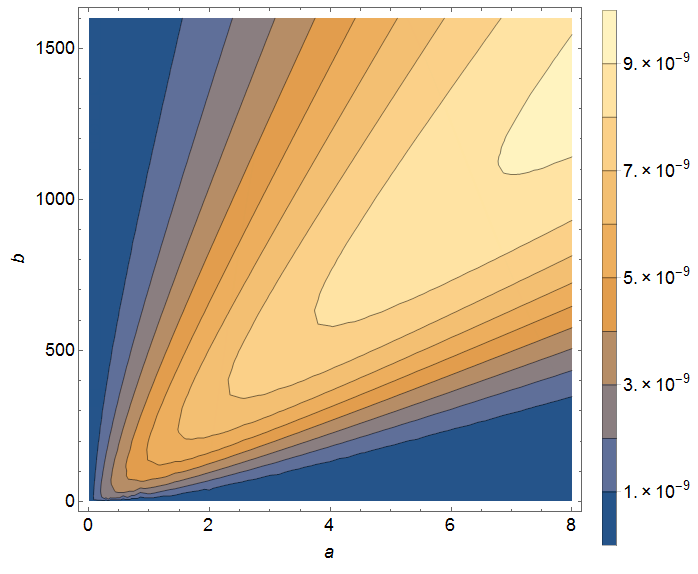
\includegraphics[height=2.5in]{figures/single-app-marginal-lik-contour-plot}\caption{\label{fig:single-app-contour-plot}A plot of $p(\protect\cd_{i}\mid a,b)$
as a function of $a$ and $b$. }
\end{figure}
It appears from this plot that the likelihood will keep increasing
as $a$ and $b$ increase, at least if $a$ and $b$ maintain a particular
ratio. Indeed, this likelihood function never attains its maximum,
so we cannot use ML-2 here. Explain what's happening to the prior
as we continue to increase the likelihood. {[}Hint: It is a property
of the Beta distribution (not difficult to see), that for any $\theta\in\left(0,1\right)$,
there is a Beta distribution with expected value $\theta$ and variance
less than $\eps$, for any $\eps>0$. What's going in here is similar
to what happens when you attempt to fit a gaussian distribution $\cn(\mu,\sigma^{2})$
to a single data point using maximum likelihood.{]}
\\
\noindent\rule{14.3cm}{2pt}
\\
\textbf{Answer:}\\
If we keep increase the likelihood, the effect of prior on posterior will increase and finally dominate the posterior distribution. (The posterior is a beta distribution that still dominated by the a,b term)
\end{enumerate}
\pagebreak




\subsection{\label{subsec:Empirical-Bayes-multiple-apps}Empirical Bayes Using
All App Data}

In the previous section, we considered working with data from a single
app. With a fixed prior, such as Beta(3,400), our Bayesian estimates
for $\theta_{i}$ seem more reasonable to me\footnote{I say ``to me'', since I am the one who chose the prior. You may
have an entirely different prior, and think that my estimates are
terrible.} than the MLE when our sample size $n_{i}$ is small. The fact that
these estimates seem reasonable is an immediate consequence of the
fact that I chose the prior to give high probability to estimates
that seem reasonable to me, before ever seeing the data. Our earlier
attempt to use empirical Bayes (ML-2) to choose the prior in a data-driven
way was not successful. With only a single app, we were essentially
overfitting the prior to the data we have. In this section, we'll
consider using the data from all the apps, in which case empirical
Bayes makes more sense.
\begin{enumerate}
\item Let $\cd=\left(\cd_{1},\ldots,\cd_{d}\right)$ be the data from all
the apps. Give an expression for $p(\cd\mid a,b)$, the \textbf{marginal
likelihood} of $\cd$. Expression should be in terms of $a,b,x_{i},n_{i}$
for $i=1,\ldots,d$. Assume data from different apps are independent.
(Hint: This problem should be easy, based on a problem from the previous
section.) 
\\
\noindent\rule{14.3cm}{2pt}
\\
\textbf{Answer:}\\
\begin{align}
p(\cd \mid a,b) &= \prod_{i=1}^d p(\cd_i \mid a,b)\\
&=\prod_{i=1}^d \frac{B(x_i+a,n_i-x_i+b)}{B(a,b)}
\end{align}


\pagebreak
\item Explain why $p(\theta_{i}\mid\cd)=p(\theta_{i}\mid\cd_{i})$, according
to our model. In other words, once we choose values for parameters
$a$ and $b$, information about one app does not give any information
about other apps.
\\
\noindent\rule{14.3cm}{2pt}
\\
\textbf{Answer:}\\
By bayes rule
\begin{equation}
p(\theta_i \mid \cd) =\frac{ p(\cd \mid \theta_i)p(\theta_i)}{p(\cd)}=\frac{ p(\cd \mid \theta_i)p(\theta_i)}{\prod_{k=1}^p p(\cd_k)}
\end{equation}
$p(\theta_i)$ is the prior on $\theta_i$ that depends only on a and b, which is same for all i. For $p(\cd \mid \theta_i)$, we have:
\begin{equation}
p(\cd \mid \theta_i) = \prod_{k=1}^d p(\cd_k \mid \theta_i)
\end{equation}
Since $\cd_k$ only depends on $\theta_k$ for all $k$. $\theta_i$ will only affect $p(\cd_i \mid \theta_i)$ and $p(\cd_k \mid \theta_i)=p(\cd_k)$ for all $k \neq i$. Plug this result to (15) and (14) we get:
\begin{align}
p(\theta_i \mid \cd) &= \frac{p(\cd_i \mid \theta_i)p(\theta_i)\prod_{k\neq i}p(\cd_k)}{\prod_{k\neq i} p(\cd_k)p(\cd_i)}\\
&=\frac{p(\cd_i \mid \theta_i)p(\theta_i)}{p(\cd_i)}\\
&=p(\theta_i \mid \cd_i)
\end{align}
\pagebreak
\item Suppose we have data from 6 apps. 3 of the apps have a fair number
of impressions, and 3 have relatively few. Suppose we observe the
following:\\
\begin{tabular}{|c|c|c|}
\hline 
 & Num Clicks & Num Impressions\tabularnewline
\hline 
\hline 
App 1 & 50 & 10000\tabularnewline
\hline 
App 2 & 160 & 20000\tabularnewline
\hline 
App 3 & 180 & 60000\tabularnewline
\hline 
App 4 & 0 & 100\tabularnewline
\hline 
App 5 & 0 & 5\tabularnewline
\hline 
App 6 & 1 & 2\tabularnewline
\hline 
\end{tabular}\\
Compute the empirical Bayes estimates for $a$ and $b$. (Recall,
this amounts to computing $(\hat{a},\hat{b})=\argmax_{\left(a,b\right)\in\reals^{>0}\times\reals^{>0}}p(\cd\mid a,b).$)
This will require solving an optimization problem, for which you are
free to use any optimization software you like (perhaps \href{https://docs.scipy.org/doc/scipy/reference/optimize.html}{scipy.optimize}
would be useful). The empirical Bayes prior is then Beta$(\hat{a},\hat{b})$,
where $\hat{a}$ and $\hat{b}$ are our ML-2 estimates. Give the corresponding
prior mean and standard deviation for this prior.
\\
\noindent\rule{14.3cm}{2pt}
\\
\textbf{Answer:}\\
To compute the empirical Bayes estimates for $a$ and $b$, we are looking for:
\[
\argmax_{a,b} \prod_{i=1}^d \frac{B(x_i+a,n_i-x_i+b)}{B(a,b)}=\argmax_{a,b} [\sum_{i=1}^{d}\log(B(x_i+a,n_i-x_i+b))-\log(B(a,b))]
\]
The following codes are used for optimization which yields result of $a=6.469$ and $b=1181.437$. The prior mean is approximately 0.54\% with standard deviation 0.21\%:
\begin{minted}{python}
import numpy as np
import scipy
from scipy.special import beta,betaln
from scipy.misc import comb
from scipy.optimize import minimize

#data
x = [50,160,180,0,0,1]
n = [10000,20000,60000,100,5,2]

#Likelihood function
def pD(ab):
    assert len(ab)==2
    cumSum_list = []
    a = ab[0]
    b = ab[1]
    for i in range(len(x)):
        xi = x[i]
        ni = n[i]
        #print(beta(xi+a,ni-xi+b))
        #cumProd_list.append(comb(k=xi,N=ni,exact=True)*beta(xi+a,ni-xi+b)/beta(a,b))
        cumSum_list.append(betaln(xi+a,ni-xi+b)-betaln(a,b))
    return -np.cumsum(cumSum_list)[-1]
#optimization
x0 = [8,1000]
minimize(fun=pD,x0=x0,method='Nelder-Mead',)

#optimization result
final_simplex: (array([[    6.46896461,  1181.43722485],
   [    6.46896415,  1181.43714184],
   [    6.46896422,  1181.43715013]]), array([ 2483.72514115,  2483.72514115,  2483.72514115]))
       fun: 2483.7251411499501
   message: 'Optimization terminated successfully.'
      nfev: 104
       nit: 48
    status: 0
   success: True
         x: array([    6.46896461,  1181.43722485])
\end{minted}

\pagebreak
\item Complete the following table:\\
\begin{tabular}{|c|c|c|c|c|c|c|}
\hline 
 & NumClicks & NumImpressions & MLE & MAP & PosteriorMean & PosteriorSD\tabularnewline
\hline 
\hline 
App 1 & 50 & 10000 & 0.5\%  & \textbf{0.5\%} & \textbf{0.5\%} &\textbf{0.07\%} \tabularnewline
\hline 
App 2 & 160 & 20000 & 0.8\%  & \textbf{0.78\%} & \textbf{0.79\%} & \textbf{0.06\%}\tabularnewline
\hline 
App 3 & 180 & 60000 & 0.3\%  &\textbf{0.3\%}  & \textbf{0.3\%} & \textbf{0.02\%}\tabularnewline
\hline 
App 4 & 0 & 100 & 0\%  &\textbf{0.43\%}  &\textbf{0.5\%}  &\textbf{0.2\%} \tabularnewline
\hline 
App 5 & 0 & 5 & 0\%  &\textbf{0.46\%}  &\textbf{0.54\%}  &\textbf{0.21\%} \tabularnewline
\hline 
App 6 & 1 & 2 & 50\%  &\textbf{0.54\%}  &  \textbf{0.23\%}&\textbf{0.43\%} \tabularnewline
\hline 
\end{tabular}\\
Make sure to take a look at the PosteriorSD values and note which
are big and which are small.
\\
\noindent\rule{14.3cm}{2pt}
\\
\textbf{Answer:}\\
Calculation process is omitted here and the results are already been filled in the table above with bold characters.\\
\\
We can observe that the PosteriorSD are much larger for those apps with less impressions. This makes sense because we have less data for them.
\end{enumerate}


\pagebreak
\subsection{{[}Optional{]} Hierarchical Bayes}

In Section \ref{subsec:Empirical-Bayes-multiple-apps} we managed
to get empirical Bayes ML-II estimates for $a$ and $b$ by assuming
we had data from multiple apps. However, we didn't really address
the issue that ML-II, as a maximum likelihood method, is prone to
overfitting if we don't have enough data (in this case, enough apps).
Moreover, a true Bayesian would reject this approach, since we're
using our data to determine our prior. If we don't have enough confidence
to choose parameters for $a$ and $b$ without looking at the data,
then the only proper Bayesian approach is to put another prior on
the parameters $a$ and $b$. If you are very uncertain about values
for $a$ and $b$, you could put priors on them that have high variance. 
\begin{enumerate}
\item {[}Optional{]} Suppose $P$ is the Beta$(a,b)$ distribution. Conceptually,
rather than putting priors on $a$ and $b$, it's easier to reason
about priors on the mean $m$ and the variance $v$ of $P$. If we
parameterize $P$ by its mean $m$ and the variance $v$, give an
expression for the density function $\mbox{Beta}(\theta;m,v)$. You
are free to use the internet to get this expression \textendash{}
just be confident it's correct. {[}Hint: To derive this, you may find
it convenient to write some expression in terms of $\eta=a+b$.{]}
\pagebreak
\item {[}Optional{]} Suggest a prior distribution to put on $m$ and $v$.
{[}Hint: You might want to use one of the distribution families given
\href{https://davidrosenberg.github.io/mlcourse/Archive/2016/Lectures/10b.conditional-probability-models.pdf\#page=6}{in this lecture}.
\pagebreak
\item {[}Optional{]} Once we have our prior on $m$ and $v$, we can go
``full Bayesian'' and compute posterior distributions on $\theta_{1},\ldots,\theta_{d}$.
However, these no longer have closed forms. We would have to use approximation
techniques, typically either a Monte Carlo sampling approach or a
variational method, which are beyond the scope of this course\footnote{If you're very ambitious, you could try out a package like \href{https://pystan.readthedocs.io/en/latest/}{PyStan}
to see what happens.}. After observing the data $\mbox{\ensuremath{\cd}}$, $m$ and $v$
will have some posterior distribution $p(m,v\mid\cd)$. We can approximate
that distribution by a point mass at the mode of that distribution
$\left(m_{\text{MAP}},v_{\text{MAP}}\right)=\argmax_{m,v}p(m,v\mid\cd)$.\textbf{
Give expressions} for the posterior distribution $p(\theta_{1},\ldots,\theta_{d}\mid\cd)$,
with and without this approximation. You do not need to give any explicit
expressions here. It's fine to have expressions like $p(\theta_{1},\ldots,\theta_{d}\mid m,v)$
in your solution. Without the approximation, you will probably need
some integrals. It's these integrals that we need sampling or variational
approaches to approximate. While one can see this approach as a way
to approximate the proper Bayesian approach, one could also be skeptical
and say this is just another way to determine your prior from the
data. The estimators $\left(m_{\text{MAP}},v_{\text{MAP}}\right)$
are often called \textbf{MAP-II estimators}, since they are MAP estimators
at a higher level of the Bayesian hierarchy.  
\end{enumerate}
\pagebreak
\section{Bayesian Linear Regression}

In this problem, we will implement Bayesian Gaussian linear regression,
essentially reproducing the example \href{https://davidrosenberg.github.io/mlcourse/Archive/2016/Lectures/13a.bayesian-regression.pdf\#page=12}{from lecture},
which in turn is based on the example in Figure 3.7 of Bishop's \emph{Pattern
Recognition and Machine Learning} (page 155). We've provided plotting
functionality in \textquotedbl{}support\_code.py\textquotedbl{}. Your
task is to complete \textquotedbl{}problem.py\textquotedbl{}. The
implementation uses np.matrix objects, and you are welcome to use\footnote{However, in practice we are usually interested in computing the product
of a matrix inverse and a vector, i.e. $X^{-1}b$. In this case, it's
usually faster and more accurate to use a library's algorithms for
solving a system of linear equations. Note that $y=X^{-1}b$ is just
the solution to the linear system $Xy=b$. See for example \href{https://www.johndcook.com/blog/2010/01/19/dont-invert-that-matrix/}{John Cook's blog post}
for discussion. } the np.matrix.getI method. 
\begin{enumerate}
\item Implement likelihoodFunc.
\\
\noindent\rule{14.3cm}{2pt}
\\
\textbf{Answer:}\\
A major draw back of the following codes is the implementation of for loop. I did try to leverage scipy.stats.multivariate\_normal.pdf but it behaves strangely Sorry for not having enough time to investigate.
\begin{minted}{python}
def likelihoodFunc(W, x, y_train, likelihood_var):
    '''
    Implement likelihoodFunc. This function returns the data likelihood
    given f(y_train | x; W) ~ Normal(w^Tx, likelihood_var).

    Args:
        W: Weights
        x: Training design matrix with first col all ones (np.matrix)
        y_train: Training response vector (np.matrix)
        likelihood_var: likelihood variance

    Returns:
        likelihood: Data likelihood (float)
    '''
    likelihood = 1
    for i in range(len(x)):
        mu = np.dot(W.T, x[i, :].T)
        likelihood *= 1 / np.sqrt(2 * math.pi * likelihood_var) * np.exp((-(y_train[i] - mu) ** 2 / (2 * likelihood_var)))
    return likelihood
\end{minted}
\pagebreak
\item Implement getPosteriorParams.
\\
\noindent\rule{14.3cm}{2pt}
\\
\textbf{Answer:}\\
This code should work with the problem.py set up which has prior mean of zero and uncorrelated features. 
\begin{minted}{python}
def getPosteriorParams(x, y_train, prior, likelihood_var = 0.2**2):
    '''
    Implement getPosterioParams. This function returns the posterior
    mean vector \mu_p and posterior covariance matrix \Sigma_p for
    Bayesian regression (normal likelihood and prior).

    Note support_code.make_plots takes this completed function as an argument.

    Args:
        x: Training design matrix with first col all ones (np.matrix)
        y_train: Training response vector (np.matrix)
        prior: Prior parameters; dict with 'mean' (prior mean np.matrix)
               and 'var' (prior covariance np.matrix)
        likelihood_var: likelihood variance- default (0.2**2) per the lecture slides

    Returns:
        postMean: Posterior mean (np.matrix)
        postVar: Posterior mean (np.matrix)
    '''
    # This infact assume prior mean are all zero
    wdim = x.shape[1]
    postMean = (np.dot(x.T,x)+likelihood_var**2*prior['var'].getI()).getI().dot(x.T).dot(y_train)
    postVar = (likelihood_var**(-2)*np.dot(x.T,x)+prior['var'].getI()).getI()
    #postMean.resize(wdim)
    return postMean, postVar
\end{minted}

\pagebreak
\item Implement getPredictiveParams.
\\
\noindent\rule{14.3cm}{2pt}
\\
\textbf{Answer:}\\
\begin{minted}{python}
def getPredictiveParams(x_new, postMean, postVar, likelihood_var = 0.2**2):
    '''
    Implement getPredictiveParams. This function returns the predictive
    distribution parameters (mean and variance) given the posterior mean
    and covariance matrix (returned from getPosteriorParams) and the
    likelihood variance (default value from lecture).

    Args:
        x: New observation (np.matrix object)
        postMean, postVar: Returned from getPosteriorParams
        likelihood_var: likelihood variance (0.2**2) per the lecture slides

    Returns:
        - predMean: Mean of predictive distribution
        - predVar: Variance of predictive distribution
    '''

    # TO DO
    x_new = x_new.reshape(-1,1)
    predMean = np.dot(postMean.T,x_new)
    predVar = x_new.T.dot(postVar).dot(x_new)+likelihood_var**2
    return predMean, predVar
\end{minted}

\pagebreak
\item Run 'python problem.py' from inside the Bayesian Regression directory
to generate the plots. Note we suggest you change the default behavior
in support\_code.make\_plots from plt.show, to saving the plots for
inclusion in your homework submission.
\\
\noindent\rule{14.3cm}{2pt}
\\
\textbf{Answer:}\\
\begin{figure}[ht]
\caption{Prior variance: $\frac{1}{2}$}
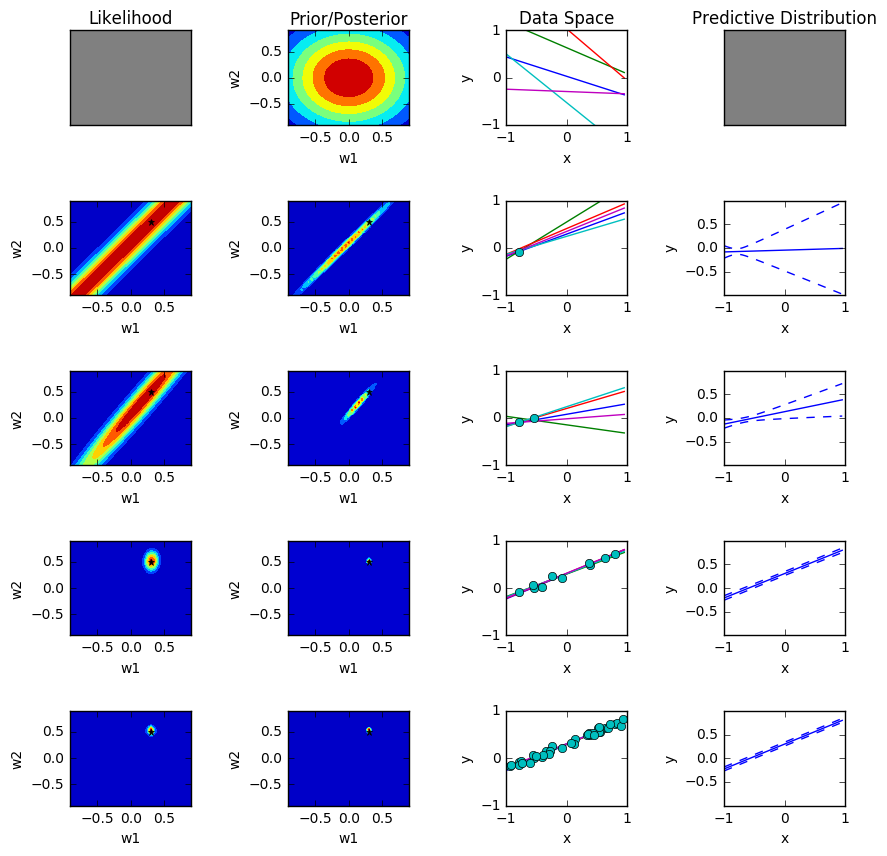
\includegraphics[width=\textwidth]{bayes_reg.png}
\end{figure}
\begin{figure}[ht]
\caption{Prior variance: $\frac{1}{2^5}$}
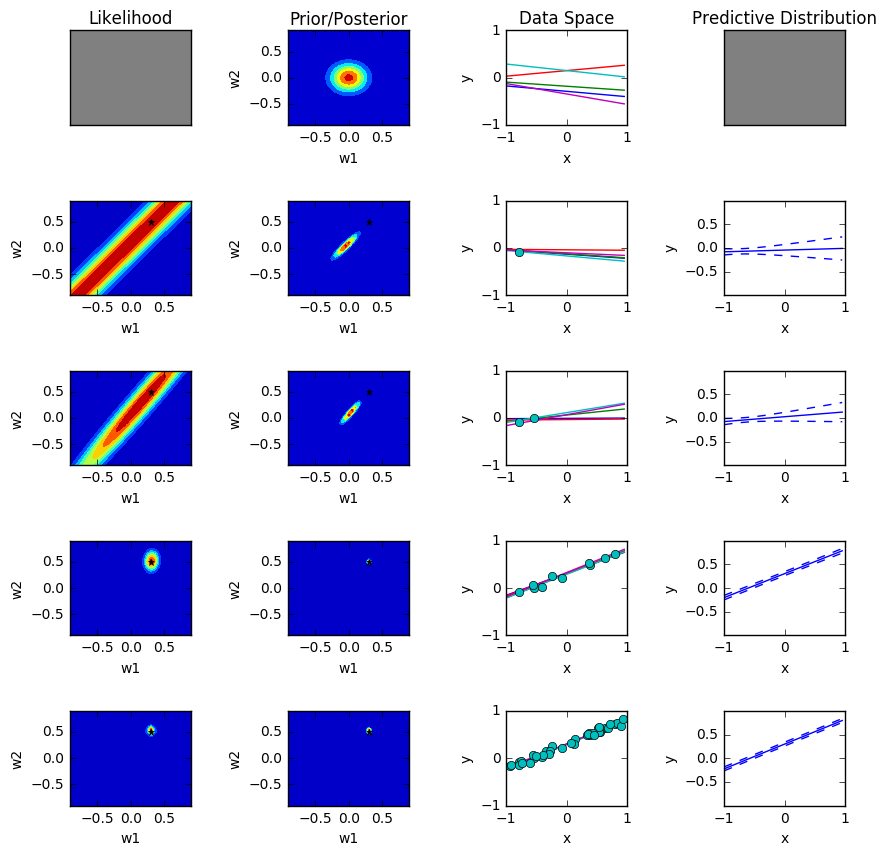
\includegraphics[width=\textwidth]{bayes_reg2.png}
\end{figure}
\begin{figure}[ht]
\caption{Prior variance: $\frac{1}{2^10}$}
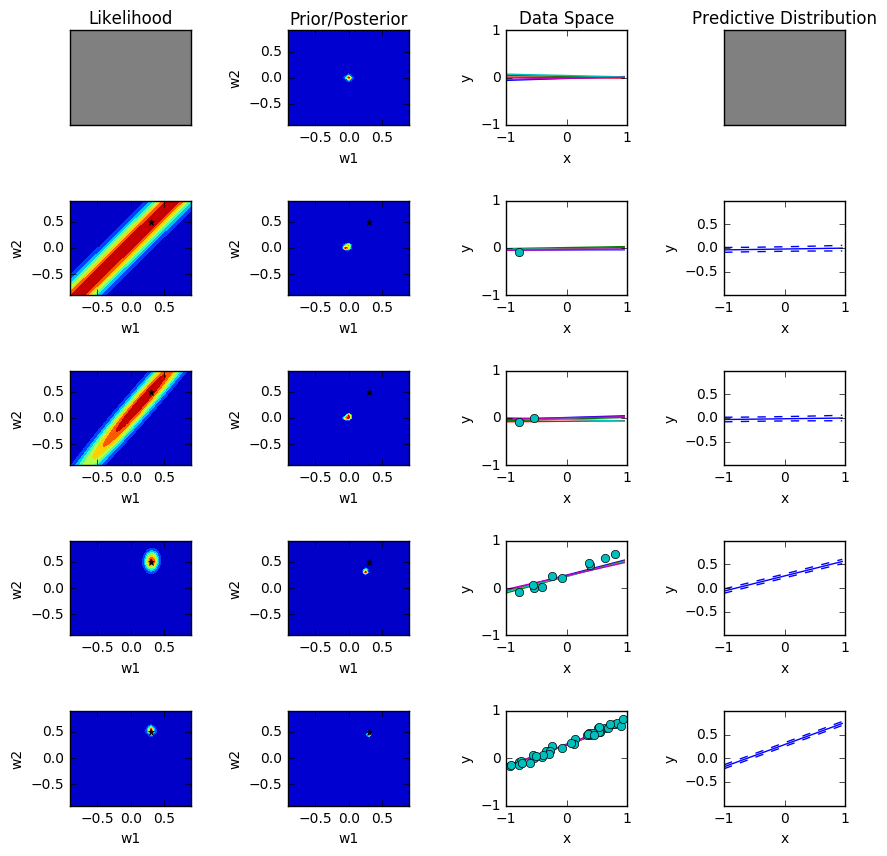
\includegraphics[width=\textwidth]{bayes_reg3.png}
\end{figure}
\pagebreak[4]
\item Comment on your results. In particular, discuss how each of the following
change with sample size and with the strength of the prior:  (i) the
likelihood function, (ii) the posterior distribution, and (iii) the
posterior predictive distribution.
\\
\noindent\rule{14.3cm}{2pt}
\\
\textbf{Answer:}\\
\begin{itemize}
\item Likelihood: The strength of prior does not affect likelihood distribution.
\item Posterior: Stronger prior would result in the posterior being closer to prior distribution and if the prior is far from the the true distribution, it takes the posterior longer to converge to real distribution.
\item Predidctive distribution: Stronge prior would make the predictive distribution to have less variance in prediction in the beginning few steps and if prior is far from the true distribution the predictive distribution converges slower if the prior is strong.
\end{itemize}

\pagebreak
\item {[}Optional{]} Our work above was very much ``full Bayes'', in that
rather than coming up with a single prediction function, we have a
whole distribution over posterior prediction functions. However, sometimes
we want a single prediction function, and a common approach is to
use the MAP estimate. As we discussed in class, for this setting,
we can get the MAP estimate using ridge regression. Use ridge regression
to get the MAP prediction function corresponding to the first prior
covariance. What value did you use for the regularization coefficient?
Why? 
\end{enumerate}

\end{document}
